 % Euclidean Distance
Roughly speaking, a function that measures the distance between two points in a set is called a \emph{metric}.\footnote{Metrics and metric spaces are examined in detail in Chapter 5 of Volume I.}
The \emph{Euclidean metric} measures the distance between two points in $\mathbb{R}^n$ with the familiar distance formula:
\[
d(\x,\y) = \sqrt{\displaystyle\sum_{i=1}^n (x_i - y_i)^2} = \| \x - \y \|_2
\]

Write a function that accepts two 1-dimensional NumPy arrays and returns the Euclidean distance between them.
Raise a \li{ValueError} if the arrays don't have the same number of entries.
\\
(Hint: NumPy already has some functions to help do this quickly.)
 % Exhaustive search method.
Write a function that solves the nearest neighbor search problem by exhaustively checking all of the distances between a given point and each point in a data set.
The function should take in a set of data points (as an $m \times k$ NumPy array, where each row represents one of the $m$ points in the data set) and a single target point (as a 1-dimensional NumPy array with $k$ entries).
Return the point in the training set that is closest to the target point and its distance from the target.

The complexity of this algorithm is $O(mk)$, where $k$ is the number of dimensions and $m$ is the number of data points.
 % KDTNode class
Import the \li{BSTNode} class from the previous lab using the following code:
\begin{lstlisting}
import sys
sys.path.insert(1, "../Trees")
from trees import BSTNode
\end{lstlisting}
%\footnote{If the file containing the \li{BSTNode} class is in a different directory than your solutions file for this lab, see \url{https://docs.python.org/2/tutorial/modules.html\#packages} for instructions on packages and imports.}
Write a \li{KDTNode} class that inherits from \li{BSTNode}.
Modify the constructor so that a \li{KDTNode} can only hold a NumPy array (of type \li{np.ndarray}).
If any other data type is given, raise a \li{TypeError}.
Create an \li{axis} attribute (set it to \li{None} or $0$ for now).

\begin{comment} % Magic methods (outdated)
\item Write the \li{__sub__} magic method so that \li{x} - \li{y} returns the Euclidean distance between the data in node \li{x} and the data in node \li{y}.

\item Write the \li{__eq__} magic method so that \li{x == y} is \li{True} if and only if \li{x} and \li{y} have the same data (Hint: \li{np.allclose()})

\item Finally, write the \li{__lt__} and \li{__gt__} magic methods so that the $<$ and $>$ operators compare the $i^{th}$ entry of the data, where $i$ is the \li{axis} attribute of the node on the \emph{right side} of the operator.
For example,

\begin{lstlisting}
>>> x = KDTNode(np.array([1,2]))
>>> y = KDTNode(np.array([3,1]))
>>> y.axis = 0            # Compare the '0th' entry of the data
>>> x < y                # True, since 1 < 3
True
>>> x > y
False

>>> y.axis = 1            # Compare the '1st' entry of the data
>>> x < y                # False, since 2 > 1
False
>>> x > y
True
\end{lstlisting}
\end{comment}
 % Implement the K-D Tree!
Finish implementing the \li{KDT} class.
\begin{enumerate}
\item Override the \li{insert()} method.
To insert a new node, find the node that should be the parent of the new node by recursively descending through the tree as in the \li{find()} method (see Figure \ref{fig:k-insert} for a geometric example).
Do not allow duplicate nodes in the tree.
Note that the \li{k} attribute will be initialized when a $k$-d tree object is instantiated.

The \li{axis} attribute of the new node will be one more than that axis of the parent node.
If the last dimension of the data has been reached, start \li{axis} over at 0.

\item % To solve the nearest neighbor search problem, create the $k$-d tree only once.
% Then use it multiple times with different target points.
To prevent a user from altering the tree, disable the \li{remove()} method.
Raise a \\ \li{NotImplementedError} if the method is called, and allow it to receive any number of arguments.
(Disabling the \li{remove()} method ensures that the $k$-d tree remains the same after it is created.
The same $k$-d tree is used multiple times with different target points to solve the nearest neighbor search problem.)
\end{enumerate}
 % K-d nearest neighbor search algorithm.
Use Algorithm \ref{alg:kdneighborz} to write a function that solves the nearest neighbor search problem by searching through your \li{KDT} object.
The function should take in a NumPy array of data and a NumPy array representing the target point.
Return the nearest neighbor in the data set and the distance from the nearest neighbor to the target point, as in Problem 2 (be sure to return a NumPy array for the neighbor).

To test your function, use SciPy's built-in \li{KDTree} object.
This structure behaves like the \li{KDT} class, but its operations are heavily optimized.
To solve the nearest neighbor problem, initialize the tree with data, then ``query'' the tree with the target point.
The \li{query()} method returns a tuple of the minimum distance and the index of the nearest neighbor in the data.

\begin{lstlisting}
>>> from scipy.spatial import KDTree

# Initialize the tree with data (in this example, use random data).
>>> data = np.random.random((100,5))
>>> target = np.random.random(5)
>>> tree = KDTree(data)

# Query the tree and print the minimum distance.
>>> min_distance, index = tree.query(target)
>>> print(min_distance)
0.309671532426

# Print the nearest neighbor by indexing into the tree's data.
>>> print(tree.data[index])
[ 0.68001084  0.02021068  0.70421171  0.57488834  0.50492779]
\end{lstlisting}
 % Postal data problem.
Write a class that performs the $k$-nearest neighbors algorithm.
The constructor should accept a NumPy array of data (the training set) and a NumPy array of corresponding labels for that data.
Use SciPy's \li{KDTree} class to build a $k$-d tree from the training set in the constructor.

Write a method for this class that accepts a NumPy array of new data points and an integer \li{k}.
Use the $k$-nearest neighbors algorithm to predict the label of the new data points.
Return a NumPy array of the predicted labels.
In the case of ties between labels, choose the label with the smaller identifier (hint: try \li{scipy.stats.mode()}).

To test your classifier, use the data file \texttt{PostalData.npz}.
This is a collection of labeled handwritten digits that the United States Postal Service has made available to the public.
This data set may be loaded by using the following command:
\begin{lstlisting}
points, testpoints, labels, testlabels = np.load('PostalData.npz').items()
\end{lstlisting}

The first entry of each array is a name, so \li{points[1]} and \li{labels[1]} are the actual points and labels to use.
Each point is an image that is represented by a flattened $28 \times 28$ matrix of pixels (so each image is a NumPy array of length 784).
The corresponding label indicates the number written and is represented by an integer.

Use \li{labels[1]} and \li{points[1]} to initialize the classifier. Use \li{testpoints[1]} for predicting output classes. Choose a random data point from \li{testpoints[1]}. Plot this point with the following code:
\begin{lstlisting}
import matplotlib.pyplot as plt
plt.imshow(img.reshape((28,28)), cmap="gray")
plt.show()
\end{lstlisting}
where \li{img} is the random data point (a NumPy array of length 784). Your plot should look similar to Figure \ref{fig:digit}.

Use your classifier to predict the label of this data point.
Does the output match the number you plotted?
Compare the output of your classifier to the corresponding label in \li{testlabels[1]}.
They should be the same.

\begin{comment}
The United States Postal Service has made a collection of labeled handwritten digits available to the public, provided in \texttt{PostalData.npz}.
Write a function that uses this data for $k$-nearest neighbor classification.
This data set may be loaded by using the following command:

\begin{lstlisting}
labels, points, testlabels, testpoints = np.load('PostalData.npz').items()
\end{lstlisting}

This contains a training set and a test set.
The first entry of each array is a name, so \li{labels[1]} and \li{points[1]} are the actual points and labels to use.
Each point is an image that is represented by a flattened $28 \times 28$ matrix of pixels (so each image is represented by a NumPy array of length 784).
The corresponding label indicates the number written, and is represented by an integer.

Use SciPy's \li{KDTree} class to build a $k$-d tree from the training set of digits. Perform the $k$-nearest neighbor algorithm on the first 50 nodes in \li{testpoints} using 1, 4, and 10 neighbors, with tie breaking implemented as described above (hint: try using \li{np.bincount()}). Calculate the accuracy of your model by comparing your output to the corresponding labels in \li{testlabels}. Return the accuracies of your model.
\end{comment}

A similar classification process is used by the United States Postal Service to automatically determine the zip code written or printed on a letter.

\begin{figure}[H]
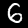
\includegraphics[width=.25\textwidth]{figures/Example.png}
\caption{The number 6 taken from the data set.}
\label{fig:digit}
\end{figure}
